\section{相关工作}


\cpar{大型多模态模型。} 长期以来的研究目标是开发能够通过多种模态感知世界的模型,类似于人类的经验。视觉和语言处理方面的最新进展已经将研究重点从较小的任务特定模型转向能够处理多样化输入的大型通用模型 \citep{team2023gemini,hurst2024gpt4o}。关键的是,预训练的视觉和语言骨干通常只需要很少的调整就能实现有效的跨模态通信 \citep{tsimpoukelli2021multimodalfrozen,shukor2023epalm,vallaeys2024improveddepalm,merullo2023linearly,koh2023grounding}。只需将视觉编码器与编码器-解码器架构 \citep{shukor2023unival,wang2022ofa,lu2022unified,mizrahi20234m} 或仅解码器的语言模型集成,就产生了高度强大的多模态系统 \citep{laurenccon2024mattersidefics2,alayrac2022flamingo,liu2024improvedllava,wang2024qwen2,xue2024xgenblip3,chen2024internvl,zhu2024minigpt,abdin2024phi3,dai2024nvlm,beyer2024paligemma,moon2024anymal}。这种后期融合方法,其中模态在组合之前被单独处理,现在已经得到了很好的理解,并且有明确的最佳实践来训练有效的模型 \citep{laurenccon2024obelics,mckinzie2025mm1,zhang2024mm1_5,lin2024vila}。相比之下,早期融合模型 \citep{fuyu8b,team2024chameleon,diao2024unveiling},在较早阶段组合模态的模型,仍然相对未被探索,只有少数公开发布的模型 \citep{fuyu8b,diao2024unveiling}。与 \citep{diao2024unveiling,team2024chameleon} 不同,我们的模型只使用一个线性层,并且完全依赖于下一个词元预测的损失。此外,我们在所有模态上从零开始训练模型,并且不进行图像的词元化。


\cpar{原生多模态模型。} 我们将那些从零开始同时在所有模态上训练的模型定义为原生多模态模型 \citep{team2023gemini},而不是通过调整语言模型以适应额外的模态。由于训练这些模型的高成本,它们仍然相对未被充分探索,大多数依赖于晚期融合架构 \citep{kosmoshuang2023language,yu2022coca}。一些从零开始训练的多模态模型 \citep{aghajanyan2022cm3,team2024chameleon,wang2024emu3} 通过利用预训练的图像词元分析器(例如 \citep{vqgan,vqvae})将图像转换为离散的词元,将其集成到文本词表中来放松这一限制。这种方法使模型能够理解和生成文本和图像,从而促进更无缝的多模态学习过程。

\cpar{缩放规律。} 缩放规律的研究旨在预测模型性能如何随训练计算量而扩展。早期工作\citep{kaplan2020scaling,hoffmann2022training}发现,大型语言模型(LLM)的性能与计算量遵循幂律关系,这使得在给定预算下能够最优估计模型参数和训练词元的数量。类似的研究已经将这些发现扩展到稀疏混合专家模型(MoE),考虑了稀疏性、专家数量和路由粒度等因素\citep{krajewski2024scalingmoe,clark2022unifiedscalingmoe,wangscalingmoe}。缩放规律还在多个领域中被观察到,包括图像模型\citep{fini2024multimodalaimv2}、视频模型\citep{rajasegaran2025empirical}、蛋白质LLMs\citep{scalingprotein}和模仿学习\citep{pearce2024scaling}。然而,很少有研究调查多模态模型的缩放规律。值得注意的是,\citet{aghajanyan2023scalingmm}研究了将模态词元化为离散词元并包含多模态生成的多模态模型。相比之下,我们专注于研究早期融合模型,该模型接受原始多模态输入并在交错的多模态数据上进行训练。




\cpar{混合专家模型 (MoE)。混合专家模型~\citep{shazeer2017outrageously} 通过将模型大小与每样本计算解耦来实现扩展模型容量,这是通过稀疏激活少量参数实现的。这种方法产生了大量稀疏模型,在训练和推理期间比密集模型更高效~\citep{fedus2022switch,sun2024hunyuan,jiang2024mixtral,liu2024deepseekv3,wei2024skywork}。
许多研究探索了从多个方面改进 MoE 大型语言模型 (LLMs),例如负载均衡、路由、稳定性、扩展性和粒度~\citep{lewis2021base,zoph2022st,lepikhin2020gshard}。然而,关于将 MoEs 应用于多模态模型的研究有限,有些工作专注于对比图像-文本模型~\citep{mustafa2022multimodal} 和后期融合多模态 LLMs~\citep{lin2024moe,li2024aria}。此外,一些研究调查了预定义专家路由,其中某些参数被保留以处理特定模态~\cite {bao2021vlmo,chen2024eve,shen2023scaling}。我们专注于研究原生早期融合模型的 MoEs,而不是提出新的架构。}




\begin{figure}[t!]
    \centering
    \captionsetup{type=figure}
    \begin{subfigure}[h]{0.95\linewidth}
    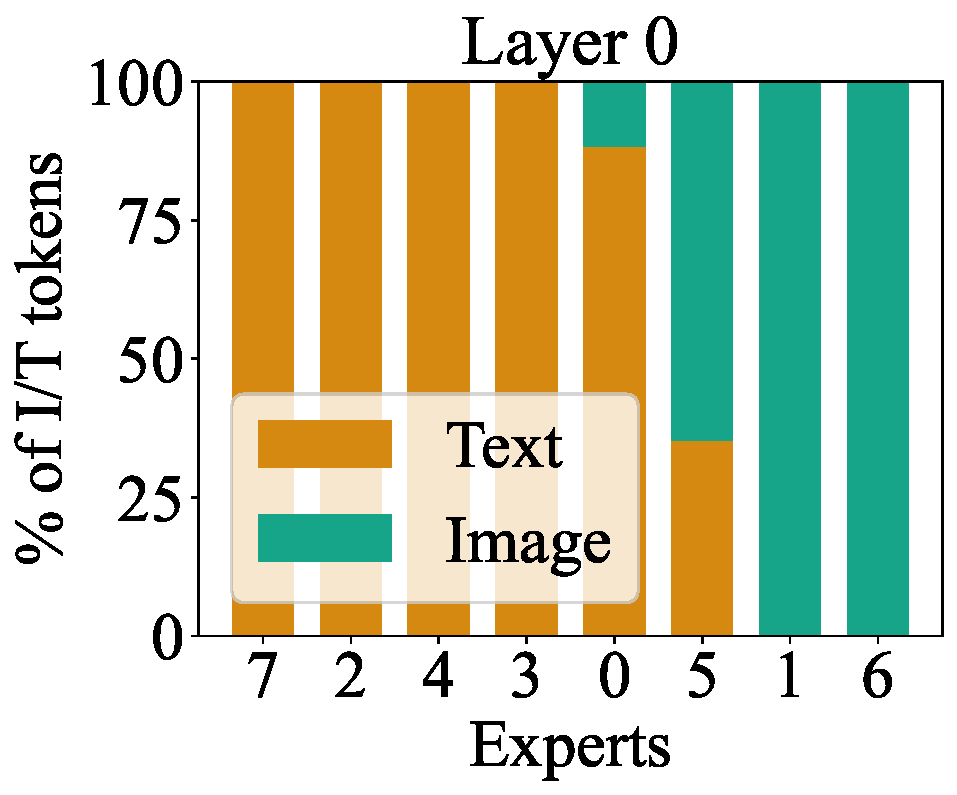
\includegraphics[height=0.27\textwidth]{assets/moes/specialization/sorted/tokens_assignment_obelics_1088_150_0.pdf}
    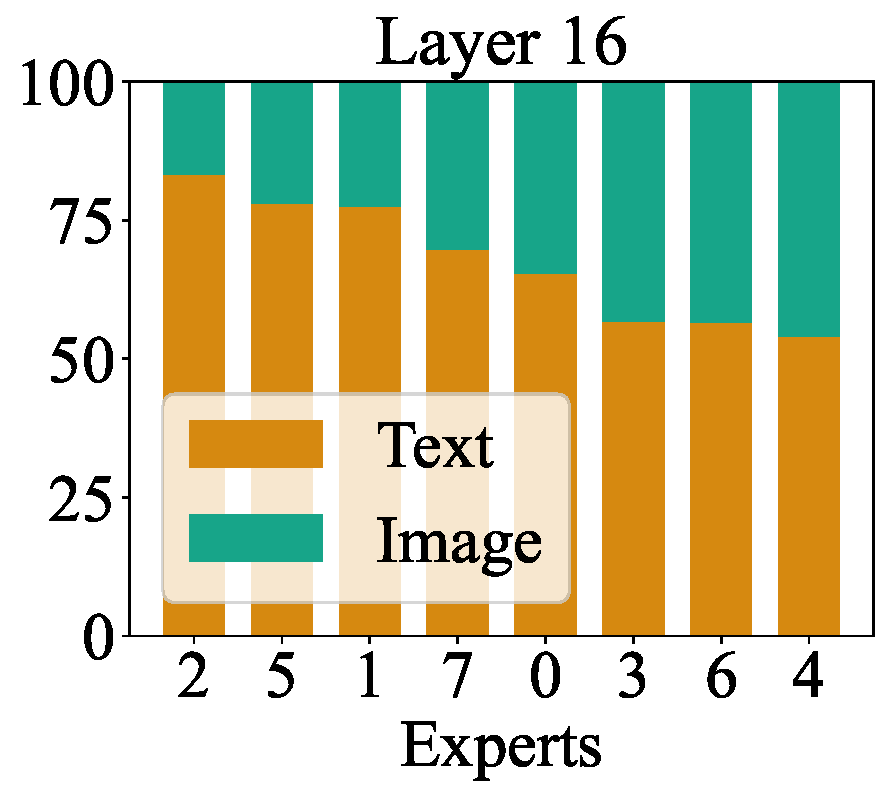
\includegraphics[height=0.27\textwidth]{assets/moes/specialization/sorted/tokens_assignment_obelics_1088_150_16.pdf}
    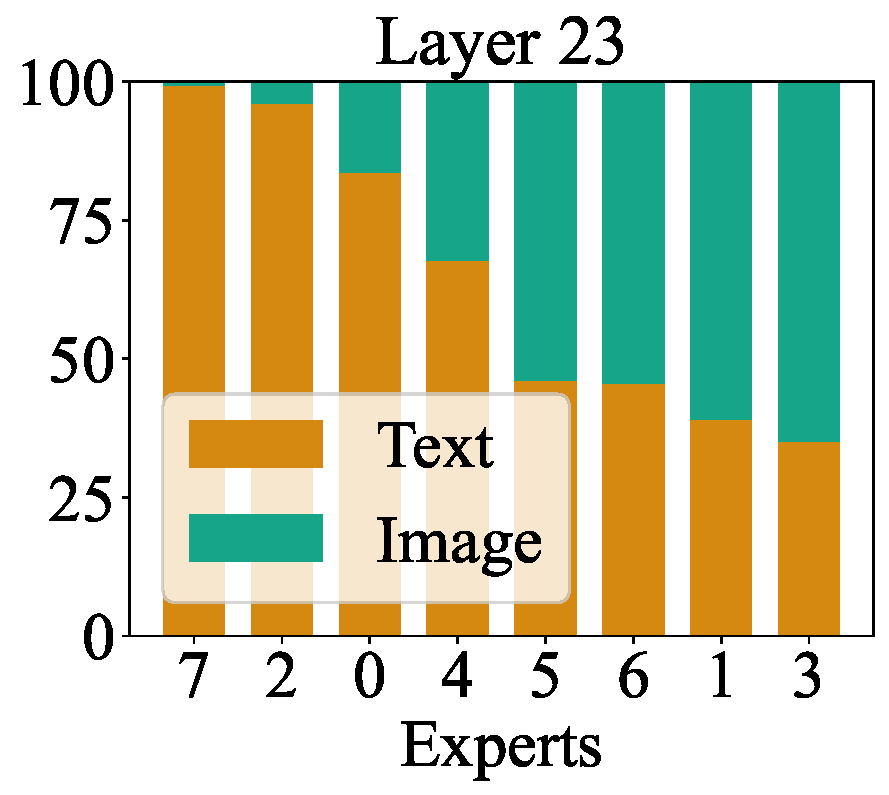
\includegraphics[height=0.27\textwidth]{assets/moes/specialization/sorted/tokens_assignment_obelics_1088_150_23.pdf}
    \end{subfigure}    \caption{\textbf{MoE 特化频率。} 从 Obelics 的交错数据中,路由到每个专家的文本和图像词元的百分比。专家按顺序排列以获得更好的可视化效果。第一层显示了最多的单峰值专家。}
    \label{fig:tokens_assignment}
\end{figure}

